
The effective efficiencies and smearing matrices are crucial inputs to the cross section, and are produced from Monte Carlo simulation.
The efficiencies and smearing matrices showed minimal model dependence in fake data tests and in our systematic uncertainty evaluation.

As an example, the efficiency as a function of muon momentum is shown in Fig.~\ref{fig:eff_mumom} and the equivalent smearing matrix is shown in Fig.~\ref{fig:migmat_mumom}.  Plots for the other primary variables and the smearing matrices are found in the Appendix.  
Efficiency values peak at roughly 35\% for all variables; this limit is primarily caused by the need to suppress cosmic-ray background and identify stopping protons.
Good efficiency is seen for proton with a momentum above 300 MeV/c (see Fig.~\ref{fig:eff_pmom}). The appendix contains figures that demonstrate the relatively high efficiency of wide angle tracks, giving the analysis $4\pi$ coverage of outgoing particles from interactions.

\begin{figure}
    \centering
    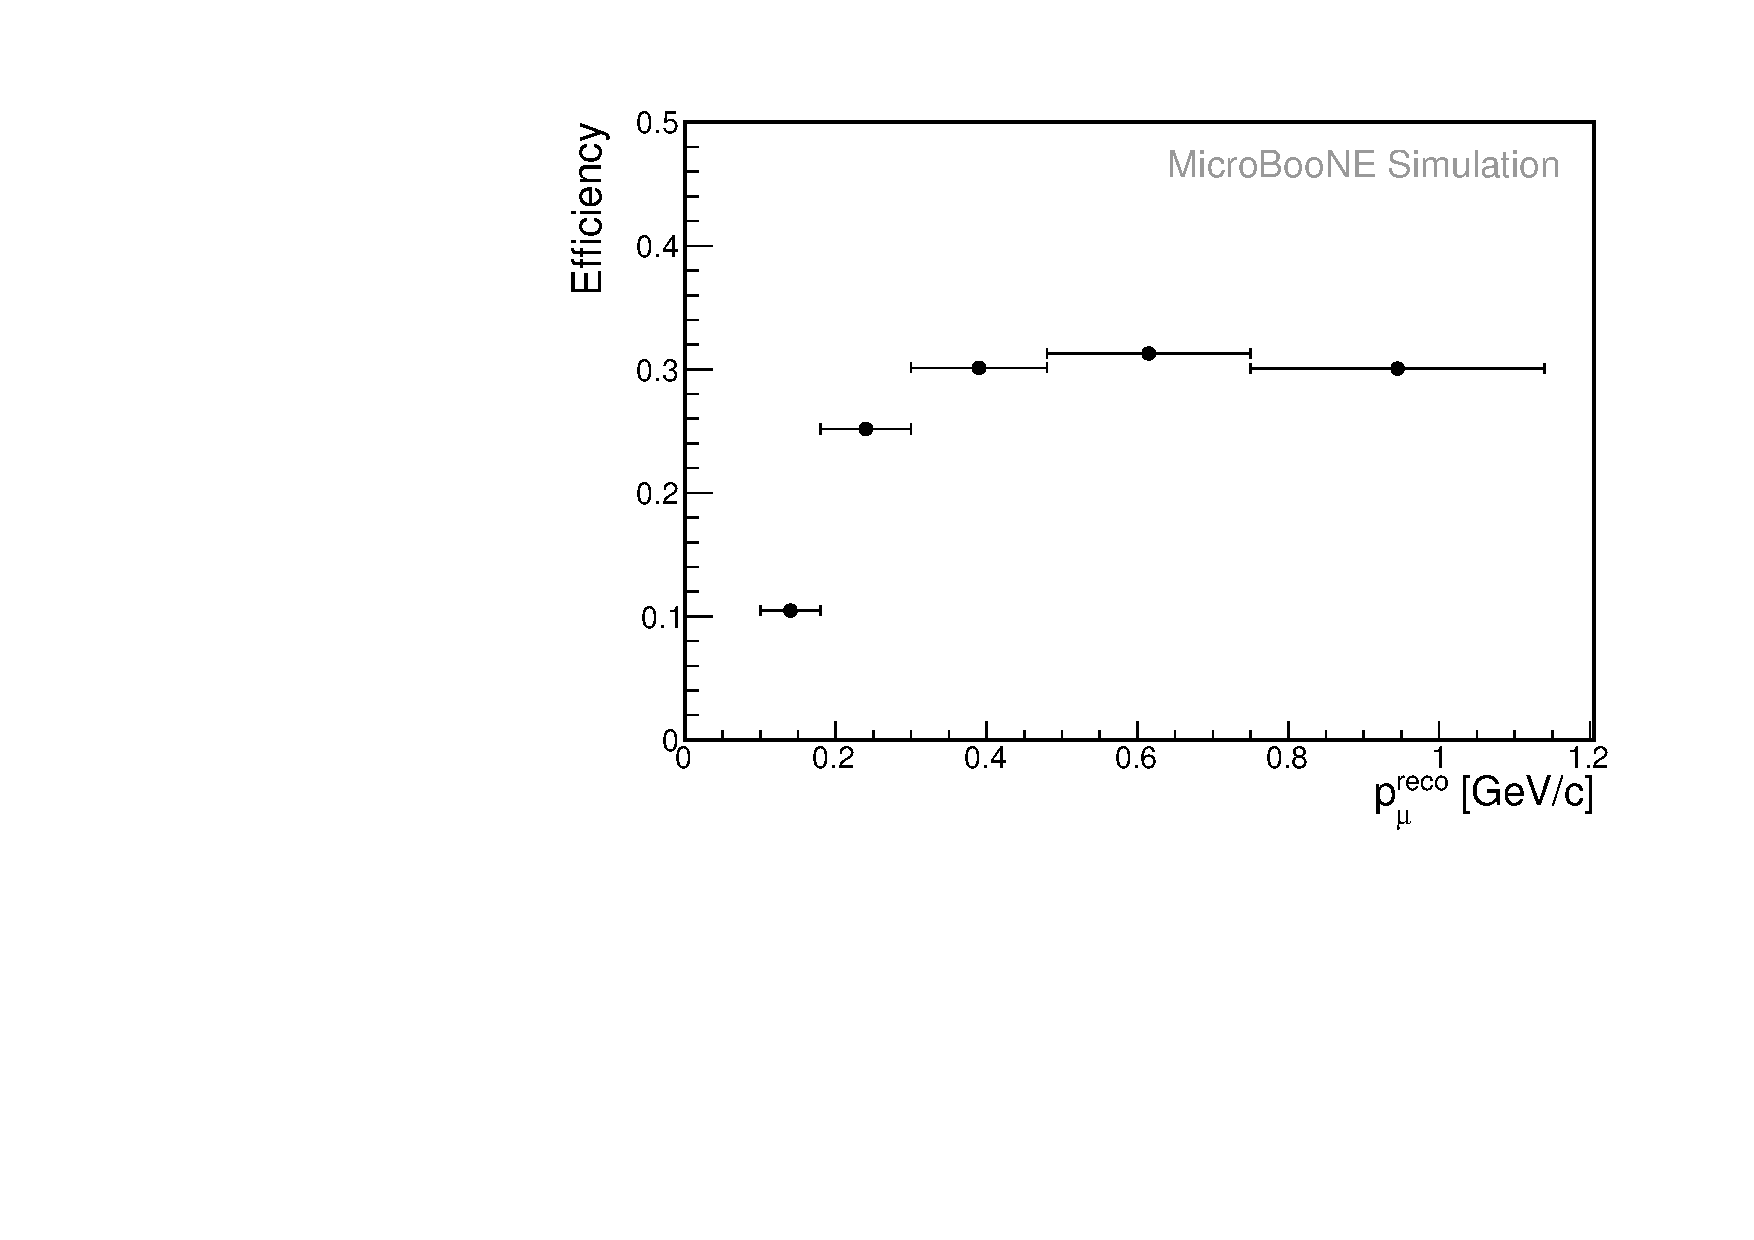
\includegraphics[width=0.45\textwidth]{Efficiency_Reco_Apr27/eff_mumom_4aug.pdf}
    \caption{Efficiency as a function of reconstructed $p_\mu$ in simulated CC$0\pi Np$ events.  Statistical error bars are too small to be seen.}
    \label{fig:eff_mumom}
\end{figure}

\begin{figure}[h!]
    \centering
    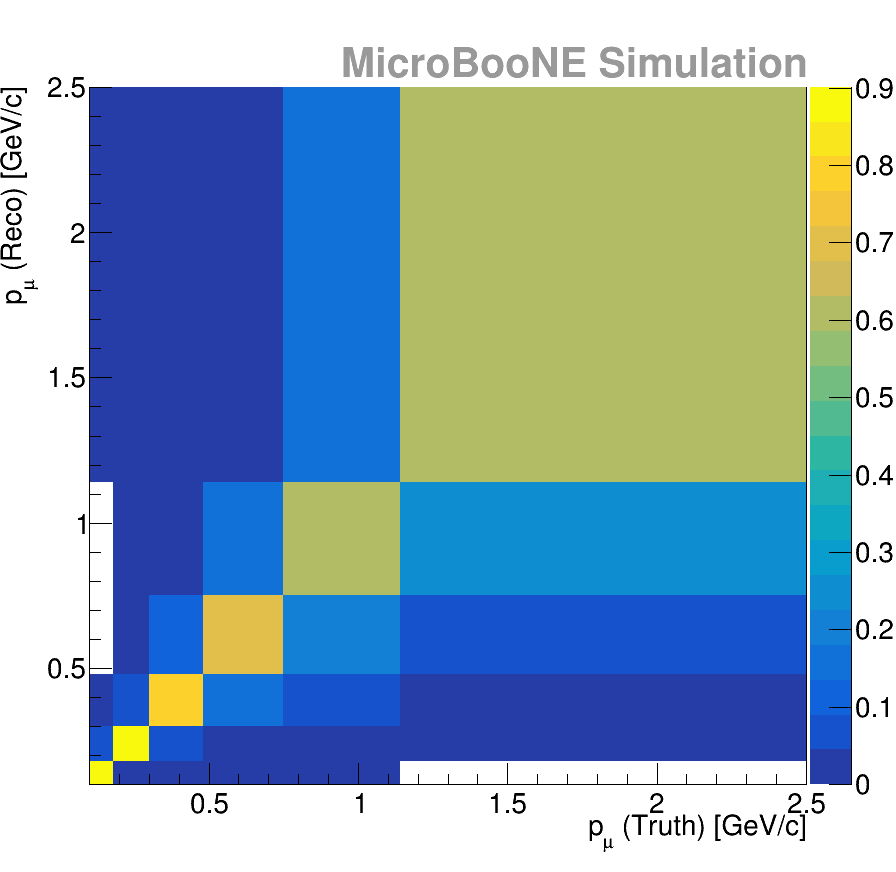
\includegraphics[width=0.45\textwidth]{MigrationMatrix0501/Fractional_MigrationMatrix_trkmom.png}
    \caption{Migration matrix between true and reconstructed bins for reconstructed muon momentum ($p_\mu$) in simulated CC$0\pi Np$ events.}
    \label{fig:migmat_mumom}
\end{figure}
